\documentclass[tikz,border=2mm]{standalone}
\usepackage{amsmath}
\usepackage{fontspec}
\setmainfont{Times New Roman}
\usetikzlibrary{arrows.meta,positioning,shapes.geometric,calc}
\begin{document}
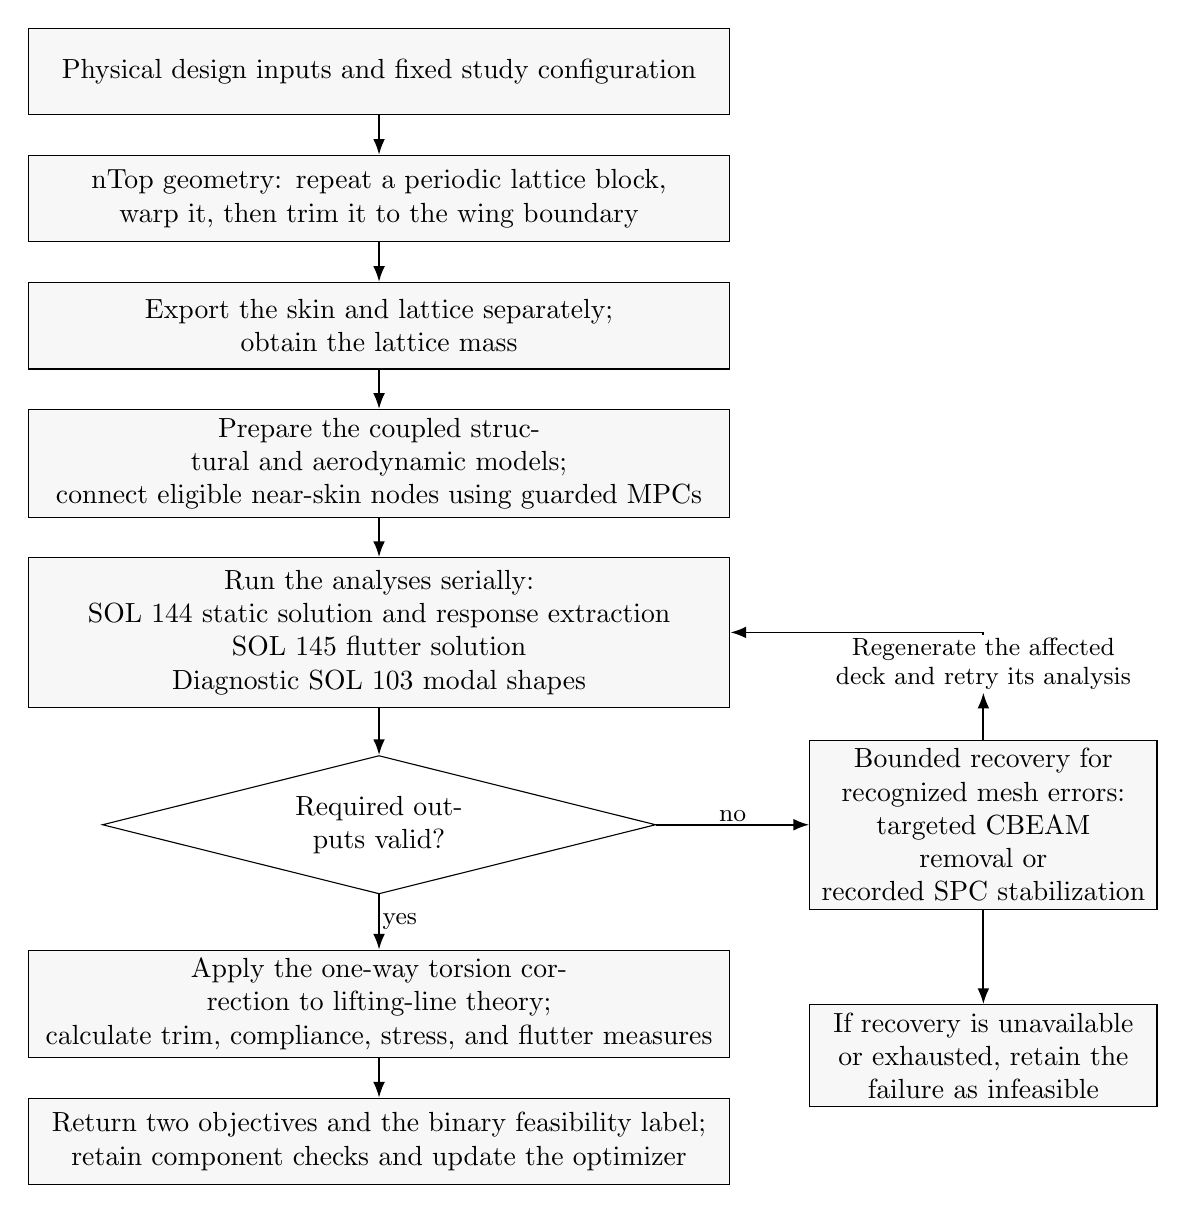
\begin{tikzpicture}[
  >={Latex[length=2mm]},
  every node/.style={font=\fontsize{10}{12}\selectfont,align=center},
  process/.style={draw,fill=black!3,text width=87mm,
    minimum height=11mm,inner sep=3pt},
  decision/.style={diamond,draw,fill=white,aspect=4.0,
    text width=36mm,inner sep=1.4pt},
  side/.style={process,text width=42mm,minimum height=12mm},
  flow/.style={->,line width=0.65pt},
  note/.style={font=\fontsize{9}{10.5}\selectfont,fill=white,inner sep=1pt}]
  \node[process] (design)
    {Physical design inputs and fixed study configuration};
  \node[process,below=5mm of design] (ntop)
    {nTop geometry: repeat a periodic lattice block,\\
    warp it, then trim it to the wing boundary};
  \node[process,below=5mm of ntop] (export)
    {Export the skin and lattice separately;\\
    obtain the lattice mass};
  \node[process,below=5mm of export] (prepare)
    {Prepare the coupled structural and aerodynamic models;\\
    connect eligible near-skin nodes using guarded MPCs};
  \node[process,below=5mm of prepare,minimum height=19mm] (analysis)
    {Run the analyses serially:\\
    SOL~144 static solution and response extraction\\
    SOL~145 flutter solution\\
    Diagnostic SOL~103 modal shapes};
  \node[decision,below=6mm of analysis] (valid)
    {Required outputs valid?};
  \node[process,below=7mm of valid] (reduce)
    {Apply the one-way torsion correction to lifting-line theory;\\
    calculate trim, compliance, stress, and flutter measures};
  \node[process,below=5mm of reduce] (record)
    {Return two objectives and the binary feasibility label;\\
    retain component checks and update the optimizer};

  \coordinate (sideanchor) at (analysis.east |- valid.center);
  \node[side,anchor=west] (recovery) at ([xshift=10mm]sideanchor)
    {Bounded recovery for\\recognized mesh errors:\\
    targeted CBEAM removal or\\recorded SPC stabilization};
  \node[note,text width=40mm,above=6mm of recovery] (retry)
    {Regenerate the affected\\deck and retry its analysis};
  \node[side,below=12mm of recovery] (failed)
    {If recovery is unavailable\\or exhausted, retain the\\failure as infeasible};

  \draw[flow] (design) -- (ntop);
  \draw[flow] (ntop) -- (export);
  \draw[flow] (export) -- (prepare);
  \draw[flow] (prepare) -- (analysis);
  \draw[flow] (analysis) -- (valid);
  \draw[flow] (valid) -- node[note,right]{yes} (reduce);
  \draw[flow] (reduce) -- (record);
  \draw[flow] (valid.east) -- node[note,above]{no} (recovery.west);
  \draw[flow] (recovery.north) -- (retry.south);
  \draw[flow] (retry.north) |- (analysis.east);
  \draw[flow] (recovery.south) -- (failed.north);
\end{tikzpicture}
\end{document}
